\documentclass{article}
\usepackage{graphicx}
\usepackage{wrapfig}
\usepackage{filecontents}
\usepackage{siunitx}
\usepackage[table]{xcolor}
\usepackage{float}
\usepackage{hyperref}
\usepackage{color} % balíček pro obarvování textů
\usepackage{xcolor}  % zapne možnost používání barev, mj. pro \definecolor
\hypersetup{
    colorlinks,
    linkcolor={red!50!black},
    citecolor={green!50!black},
    urlcolor={blue!80!black}
}
\definecolor{orange}{RGB}{ 251, 114, 032}
\definecolor{fialova}{RGB}{ 255, 000, 255} 


\usepackage[total={175mm,230mm}, top=23mm, left=20mm, includefoot]{geometry}
\usepackage{pgfplots} % http://www.chiark.greenend.org.uk/doc/texlive-doc/latex/pgfplots/pgfplots.pdf
\usepackage{blindtext}

\usepackage{subfiles} % Best loaded last in the preamble

\usepackage{bookmark}
\usepackage{tikz}
\usetikzlibrary{patterns}

\usepgfplotslibrary{polar}
\usepgfplotslibrary{external}
\usepgfplotslibrary{fillbetween}

\begin{document}
\pgfplotsset{width=140mm,compat=1.9}
\begin{figure}
    \centering
    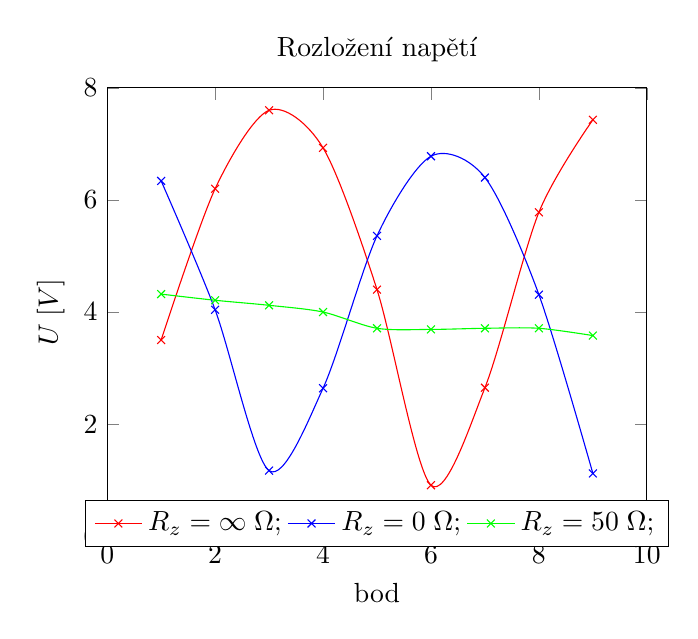
\begin{tikzpicture}
    \begin{axis}[
        title={Rozložení napětí},
        ylabel={\(U\;[V]\)},
        xlabel={bod},
        xmin=0, xmax=10,
        ymin=0, ymax=8,
        legend style={
            % area legend,
            at={(0.5,0.08)},
            anchor=north,
            legend columns=-1}]
    ]
    \addplot[
        smooth,
        color=red,
        mark=x,
        ]
        coordinates {
            (1, 3.50)
            (2, 6.20)
            (3, 7.60)
            (4, 6.93)
            (5, 4.40)
            (6, 0.91)
            (7, 2.65)
            (8, 5.78)
            (9, 7.43)
            };
    \addlegendentry{\(R_z=\infty\;\Omega\);}
    \addplot[
        smooth,
        color=blue,
        mark=x,
        ]
        coordinates {
            (1, 6.34)
            (2, 4.04)
            (3, 1.17)
            (4, 2.64)
            (5, 5.36)
            (6, 6.78)
            (7, 6.40)
            (8, 4.31)
            (9, 1.12)
        };
    \addlegendentry{\(R_z=0\;\Omega\);}
    \addplot[
        smooth,
        color=green,
        mark=x,
        ]
        coordinates {
            (1, 4.32)
            (2, 4.21)
            (3, 4.12)
            (4, 4.00)
            (5, 3.71)
            (6, 3.69)
            (7, 3.71)
            (8, 3.71)
            (9, 3.58)
        };
    \addlegendentry{\(R_z=50\;\Omega\);}
    \end{axis}
\end{tikzpicture}
\end{figure}
\begin{figure}[H]
	\begin{minipage}[t]{0.5\textwidth}
        \hspace{-5mm}
        \pgfplotsset{width=90mm,compat=1.9}
        \begin{tikzpicture}
    \begin{axis}[
        title={nakrátko},
        ylabel={\(U\;[V]\)},
        xlabel={\(f\;[MHz]\)},
        legend pos=south west,
    ]
    \addplot[
        smooth,
        color=red,
        mark=x,
        ]
        coordinates {
            (5.0, 1.58)
            (5.2, 1.90)
            (5.4, 2.26)
            (5.6, 2.67)
            (5.8, 2.97)
            (6.0, 3.12)
            (6.2, 3.38)
            (6.4, 3.42)
            (6.6, 3.25)
            (6.8, 3.10)
            (7.0, 2.85)
            (7.2, 2.61)
            (7.4, 2.48)
            (7.6, 2.29)
            (7.8, 2.15)
            (8.0, 1.99)
            (8.2, 1.86)
            (8.4, 1.73)
            (8.6, 1.62)
            (8.8, 1.52)
            };
    \end{axis}
\end{tikzpicture}
    \end{minipage}
    \hfill
	\begin{minipage}[t]{0.5\textwidth}
        \hspace{5mm}
        \pgfplotsset{width=90mm,compat=1.9}
        \begin{tikzpicture}
    \begin{axis}[
        title={naprázdno},
        ylabel={\(U\;[V]\)},
        xlabel={\(f\;[MHz]\)},
        legend pos=south west,
    ]
    \addplot[
        smooth,
        color=red,
        mark=x,
        ]
        coordinates {
            (5.0+6, 2.15)
            (5.2+6, 2.46)
            (5.4+6, 2.82)
            (5.6+6, 3.27)
            (5.8+6, 3.71)
            (6.0+6, 4.18)
            (6.2+6, 4.80)
            (6.4+6, 5.28)
            (6.6+6, 5.70)
            (6.8+6, 5.98)
            (7.0+6, 6.00)
            (7.2+6, 5.81)
            (7.4+6, 5.49)
            (7.6+6, 5.19)
            (7.8+6, 4.85)
            (8.0+6, 4.41)
            (8.2+6, 4.06)
            (8.4+6, 3.80)
            (8.6+6, 3.52)
            (8.8+6, 3.32)
            };
    \end{axis}
\end{tikzpicture}
    \end{minipage}
\end{figure}
\end{document}
